\section{Cost-quality comparison}\label{section:results-cost-quality-comparison}

This section reports the central result of \textbf{RQ3}: whether the agreement cascade is worth its cost. The cascade configuration selected in Section~\ref{section:results-abc-calibration} is placed on a strict-F1-vs-cost frontier, and is compared against each voter model within the cascade run alone. As in Section~\ref{section:results-abc-calibration}, all scores are produced by offline replay against Opus silver labels, so no API calls are made.

\medskip{}

\textbf{Cost model.} Cost is calculated by price-weighted per-tier invocation counts per chunk. For each tier, the price is the sum of its voters' input and output prices combined. The total cost of a cascade run is then computed by multiplying each tier's invocation counts with its total price, summing across tiers, and dividing by the number of chunks. For the 5-voter cascade, which was found to be the best voter subset in Section~\ref{section:results-abc-calibration}, the dropped Haiku model is excluded from the L2 tier cost, reflecting the shipped voter set.

\medskip{}

\textbf{The cascade's own frontier (E09).} For the cascade's own cost-quality frontier, the same voter set, scorer, and routing policy are kept fixed; only the agreement threshold $\theta$ is swept in this experiment. 

As shown in Table~\ref{tab:results-cascade-cost-quality-frontier}, the frontier's strict-F1 increases monotonically as $\theta$ increases, but with clear diminishing returns: moving from the \texttt{economy} point to the \texttt{knee} ($\theta = 0.8$) produces a large gain in quality, whereas moving from the \texttt{knee} ($\theta = 0.8$) to \texttt{quality} ($\theta = 0.9$) achieves a gain of 1\% strict-F1, while increasing costs by approximately 8.5\%. Escalation, therefore, is the main cost driver; most of the possible quality can be reached before the cascade approaches full escalation.

\begin{table}[htpb]
\caption[Cascade cost--quality frontier]{Representative operating points on the five-voter cascade cost--quality frontier.}
    \label{tab:results-cascade-cost-quality-frontier}
    \centering
    \begin{tabular}{l c c r r}
    \toprule
    Operating point & $\theta$ / $\theta_{\mathrm{reject}}$ & Strict F1 & Cost / chunk & Escalation \\
    \midrule
    Economy & 0.3 / 0.0 & 0.5433 & 3.38 & 0.07 \\
    Knee & 0.8 / 0.2 & 0.7067 & 21.80 & 0.87 \\
    Quality & 0.9 / 0.2 & 0.7160 & 23.66 & 0.96 \\
    \bottomrule
\end{tabular}
\end{table}

\medskip{}

\textbf{Cascade versus single models (E10).} For the single-model comparisons, all 7 voters were run alone without any cascade voting or escalation, and were scored against Opus silver labels. Table~\ref{tab:results-cascade-vs-single-model-baselines} reports the resulting strict-F1 scores and costs per chunk, for the 5-voter cascade and each of the 7 voters.

\begin{table}[htpb]
\caption[Cascade versus single-model baselines]{Cost--quality comparison between the calibrated five-voter cascade and each voter model run alone.}
    \label{tab:results-cascade-vs-single-model-baselines}
    \centering
    \begin{tabular}{l r r}
    \toprule
    System & Strict F1 & Cost / chunk \\
    \midrule
    \textbf{Cascade, five voters} & \textbf{0.7160} & \textbf{23.66} \\
    Single Claude Sonnet & 0.7129 & 18.00 \\
    Single Claude Haiku & 0.6558 & 4.80 \\
    Single GPT-4.1-mini & 0.5957 & 2.00 \\
    Single Gemini Flash & 0.5761 & 2.80 \\
    Single Gemini Flash Lite & 0.5721 & 0.50 \\
    Single GPT-4o-mini & 0.5394 & 0.75 \\
    Single GPT-4.1-nano & 0.4570 & 0.50 \\
    \bottomrule
\end{tabular}
\end{table}

The cascade and Claude Sonnet both outperform the other models: cascade is the highest scoring system with 0.7160 strict-F1, compared to the strongest single-model baseline of Claude Sonnet with a 0.7129 strict-F1. However, single-Sonnet is within 0.003 strict-F1 of the cascade, while being roughly 24\% cheaper. Every other single-model is far behind: the next best single-model is Claude Haiku, trailing the cascade by more than 6 strict-F1 points. The cheaper cascade operating points shown in Figure~\ref{fig:cost-quality-plot} do not change this: the knee is dominated by single-Sonnet on both axes, and the economy point trades most of the quality away.

\begin{figure}[htpb]
  \centering
  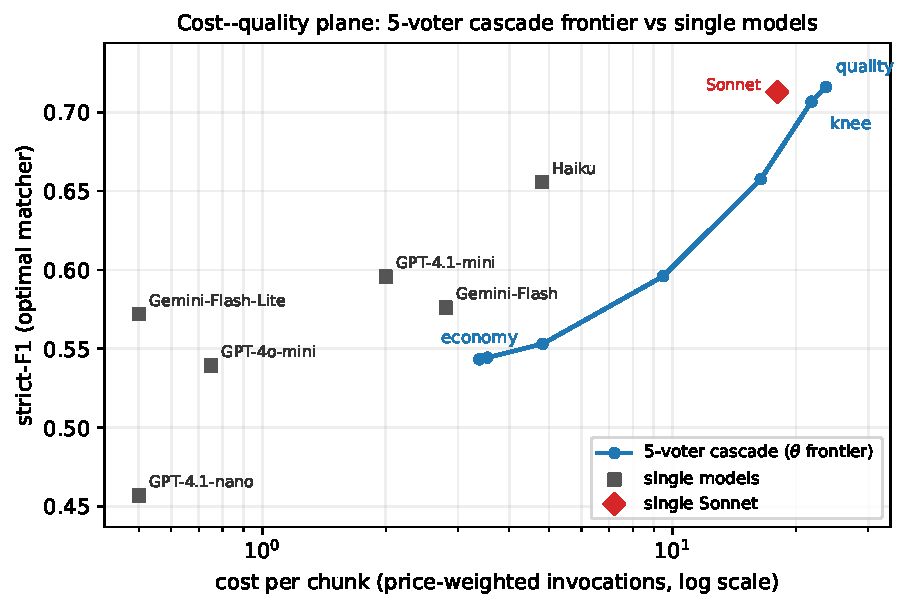
\includegraphics[width=0.72\linewidth]{figures/04_results/04_cost_quality_comparison/01_cost_quality_plane.pdf}
  \caption[Cost-quality plane: cascade
  frontier vs single models]{Strict-F1 (optimal matcher, against Opus silver) versus price-weighted cost per chunk (log scale): the five-voter cascade's economy/knee/quality $\theta$-frontier, against each voter model run alone. The cascade reaches its highest strict-F1 only at its costliest $\theta$ configuration, by a margin that is not statistically significant over the single-Sonnet baseline (Table~\ref{tab:results-bootstrap-comparison-cascade-single-models}); at every lower budget, a single model matches or beats the cascade.}
  \label{fig:cost-quality-plot}
\end{figure}

\medskip{}

\textbf{Significance (E11).} 

In order to test whether the observed differences between single-model and cascade quality are statistically significant, a paper-level clustered paired bootstrapping experiment was conducted with papers as the independent sampling unit, and $B=10000$ resamples. Table~\ref{tab:results-bootstrap-comparison-cascade-single-models} reports the strict-F1 difference between the cascade and the single-model baselines. 

The cascade significantly beats every cheaper single-model, but its difference compared to single-Sonnet is not significant: the confidence interval contains 0, showing that the cascade and single-Sonnet are statistically equivalent, while single-Sonnet is substantially cheaper to use.

\begin{table}[htpb]
\caption[Bootstrap comparison between cascade and single models]{Paper-level clustered paired bootstrap comparison between the five-voter cascade and single-model baselines.}
    \label{tab:results-bootstrap-comparison-cascade-single-models}
    \centering
    \begin{tabular}{l c c c}
    \toprule
    Cascade compared with & $\Delta$ strict-F1 & 95\% CI & Significant \\
    \midrule
    Single Claude Sonnet & +0.0031 & [$-0.0002$, $+0.0068$] & No \\
    Single Claude Haiku & +0.060 & $> 0$ & Yes \\
    Single GPT-4.1-mini & +0.120 & $> 0$ & Yes \\
    Remaining cheaper models & +0.14 to +0.26 & $> 0$ & Yes \\
    \bottomrule
\end{tabular}
\end{table}

\medskip{}

Using the cascade is \textbf{not} cost-justified against the single strong model Claude Sonnet, under the silver cost-quality criterion. Cascade outperforms all cheaper single models, but does not significantly outperform Claude Sonnet: single-Sonnet reaches a statistically equivalent strict-F1 score at a lower cost. Therefore, cascade is not the best choice if cost-quality is the only decision criterion. 

The measured gap is conservative. The silver labels are generated by Opus, and the strongest single-model baseline, Sonnet, comes from the same provider and model family, so it is structurally favored to agree with the silver standard. By contrast, once Claude Haiku is removed, the cascade's voter set is fully non-Anthropic (Section~\ref{section:results-abc-calibration}); so the findings the cascade keeps are exactly the outputs Opus-generated silver labels are least likely to reward. The observed cascade--Sonnet gap is therefore biased, if anything, against the cascade. Under the silver standard, the cascade and Sonnet are statistically indistinguishable in quality; Chapter~\ref{chapter:Discussion} discusses why the cascade may still be preferable, the shared error problem addressed by using models from multiple providers, and how a human-judged evaluation might change the picture. 

% The value the cascade provides, therefore, lies outside the strict-F1-versus-cost metric measured here. First, using a single model might share errors with the silver label model; using the cascade might catch these errors. Second, the output of the best single model Sonnet is checked against the output of the silver-label model Opus, both models from the same provider and model family: the single-Sonnet baseline is structurally favored to agree with the silver-label model. Using the cascade might help mitigate the circularity issue as well: Sonnet output is never compared to the output of the other voters, and is only used as a fallback model on voter disagreement; and with Haiku removed from the voter subset (Section~\ref{section:results-abc-calibration}), the voting that decides which chunks to accept or escalate is fully non-Anthropic. Therefore, the findings the cascade keeps reflect agreement among voters from different providers, which are exactly the outputs silver-labels generated by Opus would be least likely to reward. The measured cascade–Sonnet gap is therefore a conservative one -- biased, if anything, against the cascade.

% A human-judged quality metric could narrow, eliminate, or even reverse the small observed gap, potentially making the difference between the cascade and single-Sonnet performances statistically significant in the cascade's favor. The honest reading of the results is not that the cascade is worse, but that, under a silver standard based on the Opus output, the cascade and the single-Sonnet are statistically indistinguishable in output quality; and the case for using the cascade must rest on these two properties the cost-quality comparison cannot measure.